% !TeX root = hw.tex
\section{第零章}

\setcounter{pb}{3}
\begin{problem}
    举例说明, 整数集合 $ \mathbb{Z} $ 上存在映射 
    $ f\colon \mathbb{Z} \to \mathbb{Z} $, 使得 $ f $ 有左(右)逆但无右(左)逆。
\end{problem}

\begin{solution}
    取 $h\colon k \mapsto 2k$, 则 $g\colon 2k\mapsto k, 2k+1\mapsto 0$ 是 $h$ 的左逆. 
    因为 $h$ 非满射, 没有右逆. 这里 $g$ 有右逆 $h$, 但是非单射所以没有左逆. 分别取 $f=g, f=h$ 即可. 
\end{solution}

\begin{problem}
    试判断自反性、对称性和传递性对下列二元关系是否成立?
    \begin{enumerate}[label=(\roman*)]
        \item 实数系 $\mathbb{ R}, x - y $ 为 $ 2\pi $ 的整数倍;
        \item $\mathbb{ R}, x \geq y $;
        \item $\mathbb{ R}, x > y $;
        \item $ S $ 是仅含一个元素的集, $ x > y $。
    \end{enumerate}
\end{problem}

\begin{solution}
    关于 $S=\{\ast\}$, 此时 $>$ 视作 $S\times S$ 子集应该为空集, 对称性, 传递性成立(vacuous truth).
        \begin{table}[htbp]
            \caption{问题~\arabic{pb}}
            \centering{\begin{tabular}{|c|c|c|c|}
            \hline
                  & 反身性        & 对称性        & 传递性        \\ \hline
            (i)   & \checkmark & \checkmark & \checkmark \\ \hline
            (ii)  & \checkmark & $\times$   & \checkmark \\ \hline
            (iii) & $\times$   & $\times$   & \checkmark \\ \hline
            (iv)  & $\times$   & \checkmark & \checkmark \\ \hline
            \end{tabular}}
        \end{table}

\end{solution}

\begin{problem}
    试判断自反性、对称性和传递性对下列二元关系是否成立?
    \begin{enumerate}[label=(\roman*)]
        \item  $\mathbb{ R}, |x - y| = 1 $;
        \item $\mathbb{ R}, |x - y| \leq 1 $;
        \item $\mathbb{ R}, x - y = 1 $;
        \item $\mathbb{ R}, x + y = 1 $。
    \end{enumerate}
\end{problem}

\begin{solution}
    见下表.
    \begin{table}[htbp]
        \caption{问题~\arabic{pb}}
        \centering{\begin{tabular}{|c|c|c|c|}
        \hline
              & 反身性        & 对称性        & 传递性      \\ \hline
        (i)   & $\times$   & \checkmark & $\times$ \\ \hline
        (ii)  & \checkmark & \checkmark & $\times$ \\ \hline
        (iii) & $\times$   & $\times$   & $\times$ \\ \hline
        (iv)  & $\times$   & \checkmark & $\times$ \\ \hline
        \end{tabular}}
    \end{table}
\end{solution}

\setcounter{pb}{11}

\begin{problem}
    设$X, Y, Z$为任意集合, 又设$\psi_i:X\to Y,i=1,2,\eta:Y\to Z$. 证明:“如果$\eta\psi_1=\eta\psi_2$, 
    则$\psi_1=\psi_2$" 对任意$\psi_1,\psi_2$都成立的充要条件是$\eta$是一个单射。
\end{problem}

\begin{solution}
    充分性: 若 $\eta$ 是单射, 且 $\eta\psi_{1}=\eta\psi_{2}$, 则任意 $x\in X$ 有 $\eta(\psi_{1}(x))=\eta(\psi_{2}(x))$. 
    因为单射性, $\psi_{1}(x)=\psi_{2}(x)$ 总成立, 即 $\psi_{1}=\psi_{2}$. 
    \par 必要性: 若 $\eta$ 不是单射, 则有 $a,b\in Y$ 使得 $\eta(a)=\eta(b)$. 
    不难构造 $\psi_{1}(x)=a\ne b=\psi_{2}(x)$, 且 $\left.{\psi_{1}}\right|_{X\setminus\{x\}}^{}=\left.{\psi_{2}}\right|_{X\setminus\{x\}}^{}$. 
    则 $\eta\psi_{1}=\eta\psi_{2}$ 但是 $\psi_{1}\ne\psi_{2}$.
\end{solution}


\setcounter{pb}{15}
\begin{problem}
    应用定理 7, 证明欧拉函数$\varphi(n)$可写成
        \[
            \varphi(n)=n\sum_{d|n}\frac{\mu(d)}d.
        \]
\end{problem}

\begin{solution}
    记 $[r]=\{1,2,\dots,r\}$. 由定理~7, 对 $n=p_{1}^{e_{1}}\cdots p_{r}^{e_{r}}$, 有
        \[
            \begin{split}
                \frac{\varphi(n)}{n}
                &= (1-p_{1}^{-1})\cdots(1-p_{r}^{-1})\\
                &= \sum_{\ell=0}^{r}\sum_{\sharp\{i\mid k_{i}=1\}=\ell}(-1)^{\ell}p_{1}^{-k_{1}}\cdots p_{r}^{-k_{r}}\\
                &= \sum_{\substack{k_{i}\in\{0,1\}^{r},\\ i\in[r]}}\frac{\mu(p_{1}^{k_{1}}\cdots p_{r}^{k_{r}})}{p_{1}^{k_{1}}\cdots p_{r}^{k_{r}}}\\
                &= \sum_{\substack{d\mid n,\\ d\text{无平方因子}}} \frac{\mu(d)}{d}
                 = \sum_{d\mid n} \frac{\mu(d)}{d}.
            \end{split}
        \]
\end{solution}

\setcounter{pb}{18}

\begin{problem}
    证明:若 $f(n)$ 是一个乘性函数, 则 $h(n) = \sum_{d \mid n} \mu \big( \frac{n}{d} \big) f(d)$ 也是一个乘性函数。
\end{problem}

\begin{solution}
    对于互素的 $n_{1},n_{2}$, 有
        \[
            \begin{split}
                h(n_{1}n_{2})
                &=\sum_{d\mid n_{1}n_{2}}\mu\Big(\frac{n_{1}n_{2}}{d}\Big)f(d)=
                \sum_{\substack{d_{1}\mid n_{1},\\d_{2}\mid n_{2}}}\mu\Big(\frac{n_{1}}{d_{1}}\frac{n_{2}}{d_{2}}\Big)f(d_{1}d_{2})\\
                &=\sum_{d_{1}\mid n_{1}}\mu\Big(\frac{n_{1}}{d_{1}}\Big)f(d_{1})\sum_{d_{2}\mid n_{2}}\mu\Big(\frac{n_{2}}{d_{2}}\Big)f(d_{2})\\
                &=h(n_{1})h(n_{2}).
            \end{split}
        \]
\end{solution}

\setcounter{pb}{21}

\begin{problem}
    证明 
        \[
            \sum_{\substack{1\leq r\leq n\\ (r,n)=1}}^{}r=\frac{1}{2}n\varphi(n).
        \]
\end{problem}

\begin{solution}
    左边即对落在 $[1,n]$ 的一组 $\mathrm{mod}\ n$ 剩余类求和, 故
        \[
            \sum_{\substack{1\leq r\leq n\\ (r,n)=1}}^{}r=\sum_{\substack{1\leq r\leq n\\ (r,n)=1}}^{}n-r=\sum_{\substack{1\leq r\leq n\\ (r,n)=1}}^{}\frac{r+(n-r)}{2}=\frac{1}{2}n\varphi(n).
        \]
\end{solution}

\section{群论}
\subsection{第一章}

\setcounter{pb}{5}

\begin{problem}
    在  $S_3$ 中找出两个元素 $x,y$ , 适合  
    \[
        (xy)^2 \neq x^2 y^2.
    \]
\end{problem}

\begin{solution}
    只要 $x y\neq y x$ 即可. 取 $x=(1 2)$, $y=(1 3)$. 则 
        \[
            x y=(1 3 2)\ne y x = (1 2 3).
        \]
\end{solution}

\setcounter{pb}{8}

\begin{problem}
    证明:群 $G$ 为一交换群当且仅当映射 $x \mapsto x^{-1}$ 是一同构映射。
\end{problem}

\begin{solution}
    记 $i\colon x\mapsto x^{-1}$. $i$ 是双射. 熟知 $( x y)^{-1}=y ^{-1} x^{-1}$. 所以 $i$ 是同构当且仅当 $y^{-1}x^{-1}=x^{-1}y^{-1},\forall x,y$; 当且仅当 $x y=y x,\forall x,y$.
\end{solution}

\setcounter{pb}{13}

\begin{problem}
    设群 $G$ 的阶为一偶数, 证明 $G$ 中必有一个元素 $a \neq e$ 适合 $a^2 = e$。  
\end{problem}

\begin{solution}
    在集合 $G$ 上定义关系: $g\sim h\iff g h=e$. 则 $\sim$ 是等价关系. 
    并且, 每个等价类一定是一个元或者两个元. 
    注意 $[e]=\{e\}$ , 
        \[
            \sharp G=\sum_{[g]\in G/\sim}\sharp [g]=1+\underbracket{\sum_{\substack{[g]\in G/\sim\\ [g]\ne [e]}}\sharp [g]}_{\text{是奇数}},
        \]
    所以求和项有奇数, 即某等价类为一个元, 也即 $a^{2}=e$.
\end{solution}

\setcounter{pb}{16}

\begin{problem}
在群 $SL_2(\mathbb{Q})$ 中, 证明元素

\[
A = \begin{pmatrix} 0 & -1 \\ 1 & 0 \end{pmatrix}
\]

的阶为 $4$, 元素

\[
B = \begin{pmatrix} 0 & 1 \\ -1 & -1 \end{pmatrix}
\]

的阶为 $3$, 而 $AB$ 为无限阶元素.
\end{problem}

\begin{solution}
    直接计算
        \[
            A^{2}=\begin{pmatrix}
        -1&0\\0&-1
    \end{pmatrix},\ A^{3}=-A\ne I,\ A^{4}=I.
        \]
    于是阶为 $4$. 
        \[
            B^{2}=\begin{pmatrix}
                -1&-1\\1&0
            \end{pmatrix},\ B^{3}=\begin{pmatrix}
                1&0\\0&1
            \end{pmatrix}.
        \]
    于是阶为 $3$.
        \[
            A B=\begin{pmatrix}
                1&1\\0&1
            \end{pmatrix},\ (A B)^{n}=\begin{pmatrix}
                1&n\\0&1
            \end{pmatrix},\ \forall n\geq1.
        \]
    于是 $AB$ 为无限阶元素.
\end{solution}

\subsection{第二章}
\setcounter{pb}{21}

\begin{problem}
    证明任一非交换的 $6$ 阶群同构于 $S_3 $。
\end{problem}

\begin{solution}
    设 $G$ 为非交换 $6$ 阶群. 由 Sylow 第三定理,  
        \[
            N_{3}\coloneqq \text{Sylow $3$-子群的个数}\equiv 1\pmod3,
        \]
    且 $N_{3}\mid 2$, 可见 $N_{3}=1$. 所以有唯一一个 Sylow-$3$ 群 $P_{3}$, 且是正规子群. 
    现在, 除去子群 $P_{3}$, 还有 $3$ 个元素, 均不是 $3$ 阶元, 又不是单位元; Langrange 定理保证阶数只能从 $1,2,3,6$ 取; 
    如果有 $6$ 阶元, 那么群应是循环群, 和非交换的假设矛盾. 
    \par 取一个三阶元 $g$ , 一个二阶元 $h$; 则 $\langle g \rangle\cap \langle h \rangle=\{e\}$ 且 $\langle g,h \rangle=G$. 
    由于 $\langle g \rangle$ 是指数 $2$ 的子群, 是正规的, 也就是说 $G=\langle g \rangle \rtimes \langle h \rangle$, 有共轭作用 $\langle h \rangle \curvearrowright \langle g \rangle$, 且这个不是平凡的作用 
    (作用平凡即 $h g h^{-1}= g$, 换言之 $\langle g \rangle, \langle h \rangle$ 交换, 此时 $G$ 由他们生成从而交换). 
    非平凡的群作用对应一个非平凡的同态 $\langle h \rangle\to \operatorname{Aut}(\langle g \rangle)$, 而 $\operatorname{Aut}(\langle g \rangle)\cong \mathbb{Z}/\langle 2 \rangle$, 
    所以这共轭作用只能是
        \[
            h g h^{-1}=g^{2}, h g^{2} h^{-1}=g.
        \]
    综上所述, 
        \[
            G=\langle g,h\mid g^{3}=h^{2}=e, h g h^{-1}=g^{2}, h g^{2} h^{-1}=g \rangle;
        \]
    欲求的同构由 
        \[
            G\to S_{3} \colon g\mapsto (1 2 3),\; h\mapsto (1 2)
        \]
    给出.
\end{solution}
\begin{problem}
    定出全部互不相构的 $15$ 阶群。
\end{problem}

\begin{solution}
    由 Sylow 第三定理,  
        \[
            N_{5}\coloneqq \text{Sylow $5$-子群的个数}\equiv 1\pmod5,
        \]
    且 $N_{5}\mid 3$, 可见 $N_{5}=1$. 所以有且仅有一个 $5$ 阶正规子群 $H$. 
    同理有且仅有一个 $3$ 阶正规子群 $K$. 两个正规子群交为 $\{e\}$: $H\cap K$ 中元素阶数整除 $3,5$ 于是为 $1$. 
    计数 
        \[
            |H K|=\frac{|H||K|}{|H\cap K|}=15\implies G= H K
        \]
    由内直积的刻画, 这就是 $G=H\times K$; 换言之, $G\cong \mathbb{Z}/\langle 3 \rangle\times\mathbb{Z}/\langle 5 \rangle\cong\mathbb{Z}/\langle 15 \rangle$(中国剩余定理). 
    \par 综上所述, 同构意义下, $15$ 阶群只有 $\mathbb{Z}/\langle 15 \rangle$.
\end{solution}

% \begin{note}
%     设 $N, H $ 是 $G $ 的两个正规子群且 $N \cap H = \{e\} $, 则
%     对任意的 $x \in N, y \in H $, 有 $xy = yx$. 
%     命 $N H\to N\times H, n h\mapsto (n,h)$ 这良好定义: $n h=n'h'\implies (n,h)=(n',h')$, 则 
%         \[
%             H\ni n h n^{-1}=n' h' n^{-1}=n'n^{-1} (\underbracket{n h' n^{-1}}_{\in H})\implies n'n^{-1}\in H\implies n'n^{-1}=e.
%         \]
%     于是 $n=n', h=h'$. 以上定义出的同构 $N H\xrightarrow{\sim}N\times H$ 保证 $N,H$ 可交换. 
% \end{note}

% \begin{problem}
%     定出全部互不相构的 $10$ 阶群。
% \end{problem}

% \begin{solution}
%     % copied
%     由 Sylow 第三定理,  
%     \[
%         N_{5}\coloneqq \text{Sylow $5$-子群的个数}\equiv 1\pmod5,
%     \]
%     且 $N_{5}\mid 2$, 可见 $N_{5}=1$. 所以有一个 $5$ 阶正规子群, 设为 $H=\langle a \mid a^{5}=e\rangle$. 
%     同理 $N_{2}=1$ 或者 $N_{2}=5$. 当 $N_{2}=1$, 则类似上一题目, $G\cong \mathbb{Z}/(5)\times\mathbb{Z}/(2)$. 
%     当 $N_{2}=5$, 即有 $5$ 个 Sylow $2$-子群, 此时 $G$ 不是交换群; $Z(G)$ 即 Sylow $5$-子群. 
%     设 $K=\langle b \mid b^{2}=e \rangle$ 为一个 Sylow $2$-子群. 
    
%     则 $\operatorname{Ad}_{b}a\ne a$, 否则 $G$ 交换; 但是 $\operatorname{Ad}_{b}$ 是二阶元, 所以 $\operatorname{Ad}_{b}(a)=a^{-1}$.
%     此时 
%         \[
%             G=\langle a, b\mid a^{5}=e, b a b^{-1}=a \rangle\cong D_{5}.
%         \]
% \end{solution}

\begin{problem}
    设 $p,q $ 为不同的素数, 证明不存在阶为 $pq $ 的单群。
\end{problem}

\begin{solution}
    不妨设 $ p<q$. 由 Sylow 第三定理, $N_{q}\equiv1\pmod{q}$. 且 $N_{q}\mid p$
    所以 $N_{q}=1$, 此时 Sylow $q$-子群即正规子群.
\end{solution}

\begin{problem}
    设 $p,q $ 为不同的素数, 证明 $p^2 q $ 阶群必包含一个正规西罗子群。
\end{problem}

% \begin{itemize}
%     \item 当 $p<q$, 有 $N_{p}\equiv1\pmod{p}, N_{p}\mid q\implies N_{q}=1$; 此时 Sylow $q$-子群正规.
%     \item 当 $p>q$, 有 $N_{q}\equiv1\pmod{q}, N_{q}\mid p^{2}$: 
%     % \begin{itemize}
%     %     \item 若 $N_{q}=1$, 则 Sylow-$p$ 子群正规; 
%     %     % \item 若 $N_{q}=p$, 则 $p=1\pmod{q}$. 这 $p$ 个 Sylow $q$-子群两两仅相交于 $\{e\}$, 计数可得 $q$-阶元有 $p(q-1)$ 个. 
%     %     % 所以有 $p^{2}$ 个元,
%     %     \item 若 $N_{q}=p^{2}$, 则 $p^{2}=1\pmod{q}$. 这 $p^{2}$ 个 Sylow $q$-子群两两仅相交于 $\{e\}$, 计数可得 $q$-阶元有 $p^{2}(q-1)$ 个. 
%     %     所以有 $p^{2}-1$ 个元, 阶数从 $\{p, p^{2}, p q\}$ 中取. 若有 $p^{2}$ 阶元, 则生成 $p^{2}$ 阶子群, 即 Sylow $p$-子群, 此时 $N_{p}=1$, Sylow $p$ 子群是正规子群. 
%     %     下考虑只剩下 $p$ 阶元. 此时, $G$ 中元素阶数只取自 $\{1, p, q\}$, 可知
%     % \end{itemize}
%     % \par 
    
%     \begin{lemma}\label{lem: p^{2}q}
%         设 $G $ 为一有限群,$p $ 为 $|G| $ 的最小素因子。
%         则指数为 $p $ 的子群(如存在)必正规。    
%     \end{lemma}
    
%     \begin{proof}[引理~\ref{lem: p^{2}q} 的证明]
%         设 $G$ 是有限群, $p$ 是阶数的最小素因子, $H$ 是指数 $p$ 的子群. 则有左陪集分解
%             \[
%                 G=\bigsqcup_{i\in I}^{}g_{i}H, 
%             \]
%         这里 $|I|=[G:H] \mid |G|$, 只有 $>p$ 的素因子. 
%     \end{proof}
%     一定存在 Sylow $p$ 子群, 其指数为 $q$, $q$ 是 $p^{2}q$ 的最小素因子. 使用 Sylow $p$ 子群正规.
% \end{itemize}

% \setcounter{pb}{28}
% \begin{problem}
%     设 $G $ 为有限群, $A,B $ 是 $G $ 的两个非空子集合。如果 $|A| + |B| > |G| $, 证明 $AB = G $。
% \end{problem}


% \begin{problem}
%     设 $H $ 是有限群 $G $ 的一个非平凡的子群, 证明
%     \[
%     G \neq \bigcup_{g \in G} g H g^{-1}.
%     \]
% \end{problem}

% \setcounter{pb}{36}

% \begin{problem}
%     设群 $G $ 的阶是 $p^3 $, $p $ 为一素数。证明:若 $G $ 非交换, 则
%     \[
%     G^{(1)} = Z(G).
%     \]
% \end{problem}
\subsection{补充}

\setcounter{pb}{1}
\begin{problem}
    $k$ 是奇数,证明 $2k$ 阶群必有一个 $k$ 阶子群.
\end{problem}

\begin{vain}
    一定有 Sylow $2$-子群(同构于 $\mathbb{Z}/\langle 2 \rangle$), 设某个 Sylow $2$-子群的生成元为 $g$. 
    设 $G$ 在正则表示 $\rho$ 下有 $G \lesssim S_{n}$, 
    此时 $\rho(G)\cap A_{n}$ 是 $\rho(G)$ 的正规子群, 
    对应的 $\rho^{-1}(A_{n})$ 是 $G$ 的正规子群
\end{vain}

\setcounter{pb}{3}
\begin{problem}
    设 $G $ 是有限群,$p $ 是 $|G| $ 的最小素因子。又设 $H \leq G $ 且 $|G:H| = p $,则 $H \vartriangleleft G $。
\end{problem}

\subsection{更多习题}

\setcounter{pb}{5}

\begin{problem}
    Prove that all the groups of order $p^{2}$ is commutative. Here $p$ is a prime number.
\end{problem}

\begin{solution}
    Let $G$ be a group of order $p^{2}$. Then it has a nontrivial center, whose order is $p^{2}$ or $p$. 
    If $=p^{2}$ the $G=Z(G)$. 
    If $|Z(G)|=p$ then it is isomorphic to $\mathbb{Z}/\langle p \rangle $, let $Z(G)=\langle g \rangle$. 
    What's more, $|G\setminus Z(G)|=p^{2}-p$ elements are not in center and take $h\in G\setminus Z(G)$, which generates a subgroup $H$ of order $p$. 
    Now, 
        \[
            |Z(G) H|=\frac{|Z(G)|\times|H|}{|Z(G)\bigcap H|}=p^{2}\implies Z(G)H=G.
        \]
    Thus, $G=Z(G)\rtimes H$, and this semi-direct product is trivial, since $g\in Z(G)$ ensures $h g h^{-1}=g$. 
    Now, $G\cong (\mathbb{Z}/\langle p \rangle)^{2} $ is commutative. Therefore, it is impossible that $|Z(G)|=p$.
    \par Above all, all the groups of order $p^{2}$ is Abelian.
\end{solution}
\setcounter{pb}{8}
\begin{problem}
    Let $M $ be a finite abelian group $\neq 0$. Can $M $ be made into a left $\mathbb{Q}$-module?
\end{problem}

\begin{solution}
    It can't be made into a left $\mathbb{Q}$-module. Else, for $0\neq g\in M$, for $n\in\mathbb{Z}_{>0}$ we have $\frac{1}{n}g\in M$. 
    It turns out that $\operatorname{ord}(\frac{1}{n}g)=n \operatorname{ord}(g)$ and $\operatorname{ord}(\frac{1}{n}g)>|M|$ for large $n$, 
    which is impossible due to Langrange's Theorem.
\end{solution}

% \setcounter{pb}{8}
% \begin{problem}
%     Let $G_1 $ and $G_2 $ be simple groups. Show that every normal subgroup of $G = G_1 \times G_2 $, $\neq G $, $\neq 1 $ is isomorphic to either $G_1 $ or $G_2 $.
% \end{problem}
    
\setcounter{pb}{10}
\begin{problem}
    Determine $\operatorname{End}(\mathbb{Q},+,0)$.
\end{problem}

\begin{solution}
    作为环同构于 $\mathbb{Q}$:
        \begin{equation}
            \label{eqn: pb.grp.more.9}
            \operatorname{End}(\mathbb{Q},+,0) \to \mathbb{Q},\; f\mapsto f(1). 
        \end{equation}
    这显然是满射, 下证明是单射. 设 $f(1)=g(1)$, 则 $\forall m\in\mathbb{Z},\forall n\geq1  $, 
        \[
            \begin{split}
                & f(1)=n\cdot f\Big(\frac{1}{n}\Big)=n\cdot g\Big(\frac{1}{n}\Big)=g(1);\\
                & f\Big(\frac{m}{n}\Big)=m f\Big(\frac{1}{n}\Big)=m g\Big(\frac{1}{n}\Big)=g\Big(\frac{m}{n}\Big).
            \end{split}
        \]
    所以 $f=g$, \eqref{eqn: pb.grp.more.9} 是单射. 而同态性质: 加法层面是直接根据定义得到的, 乘法层面
        \[
            f\Big(\frac{m}{n}\Big)=\frac{m}{n}f(1)\implies(f\circ g)(1)=f( g(1) )=f(1) g(1).
        \]
\end{solution}

\setcounter{pb}{11}

\begin{problem}
    Show that any subgroup of index two is normal. Hence prove that
    $A_n$ is normal in $S_n$. 第 1 章第 12 题
    % 证明:如果在一阶为 $2n$ 的群中有一 $n$ 阶子群, 则它一定是正规子群。
\end{problem}

\begin{solution}
    Let $G$ be a group and $H\leq G$ is of index two. Then for $g\in G$, either $ g H=H$ or $G=H\sqcup g H$. 
    \begin{itemize}
        \item If $g H=H$, then $(g H)^{-1}=H g^{-1}=H^{-1}=H$ and hence $g H g^{-1}=g (H g^{-1})=g H=H$.
        \item If $G=H\sqcup g H$, then $g\notin H$ and hence $H g\neq H$; so $G=H\sqcup H g$. Compare and it follows $g H =H g$.
    \end{itemize}
    Above all, $H$ is normal.
    \par For $A_{n}$, it is known that $|A_{n}|=n!/2=|S_{n}|/2$ that is of index two and thus is normal.
\end{solution}

\begin{problem}
    Verify that the intersection of any set of normal subgroups of a group is a normal subgroup. 
    Show that if $H$ and $K$ are normal subgroups, then $HK$ is a normal subgroup.
\end{problem}


\begin{solution}
    Let $\{G_{i}\}_{i\in I}$ be a family of normal subgroups of $G$ and $\{\pi_{i}\colon G\twoheadrightarrow G/G_{i}\}$ 
    be the natural projections. Then 
        \[
            \pi\colon G \to \prod_{i\in I}G/G_{i},\; g\mapsto (\pi_{i}(g))_{i\in I}
        \]
    is a group hommorphism, whose kernel is $\ker\pi=\bigcap_{i\in I}G_{i}$, which must be a normal subgroup.
\par Let $H,K$ be normal subgroups of $G$. 
    \begin{itemize}
        \item It is a subgroup. Let $h_{1},h_{2}\in H$ and $k_{1},k_{2}\in K$, we have
            \[
                (h_{1}k_{1})^{-1}h_{2}k_{2}=k_{1}^{-1}h_{1}^{-1}h_{2}k_{2}=\underbracket{(k_{1}^{-1}h_{1}^{-1}h_{2}k_{1})}_{\in H}k_{1}^{-1}k_{2}\in H K.
            \]
        \item It is normal. Let $g\in G$, $g h k g^{-1}=(g h g^{-1}) (g k g^{-1})\in H K$ and hence $H K$ is normal.
    \end{itemize}
\end{solution}

\setcounter{pb}{15}
\begin{problem}
    Show that if $ a^m = b^m $ and $ a^n = b^n $, for $ m $ and $ n $ relatively prime positive integers, and $ a $ and $ b $ in a commutative domain, then $ a = b $.
\end{problem}

\begin{solution}
    By B\'ezout's Theorem, there are $ u,v\in\mathbb{Z}$ s.t. $u m+v n=1$. Therefore
        \[
            a=a^{u m+v n}=(a^{m})^{u}\cdot(a^{n})^{v}=(b^{m})^{u}\cdot(b^{n})^{v}=b^{u m+v n}=b.
        \]
\end{solution}

\setcounter{pb}{16}
\begin{problem}
    Determine the sign of the permutation   
    \[
    \begin{pmatrix}
    1 & 2 & \cdots & n-1 & n \\
    n & n-1 & \cdots & 2 & 1
    \end{pmatrix}
    \]
\end{problem}

\begin{solution}
    % If $n=2 k$, then
    %     \[
    %         \sigma \coloneqq 
    %         \begin{pmatrix}
    %             1 & 2 & \cdots & k & k+1 &\cdots & n-1 & n \\
    %             n & n-1 & \cdots & k+1 & k &\cdots  & 2 & 1
    %             \end{pmatrix}            ,
    %     \]
    % we see that 
    %     \[
    %         \mathrm{Inv}_{\sigma}\coloneqq \{(i,j)\mid 1\leq i<j\leq n,\ \sigma(i)>\sigma(j) \}=\bigcup_{i=1}^{n}\{(i,j)\mid i<j\leq n\}\implies\sharp\mathrm{Inv}_{\sigma}=\frac{n(n-1)}{2}.
    %     \]
    % % $\operatorname{sign}(\sigma)=(-1)^{ \sharp\mathrm{Inv}_{\sigma} }=(-1)^{k(2k-1)}=(-1)^{k}$. 
    % \par If $n=2k+1$, then 
    %     \[
    %         \sigma=    \begin{pmatrix}
    %             1 & 2 & \cdots & k+1 & \cdots & n-1 & n \\
    %             n & n-1 & \cdots& k+1 & \cdots & 2 & 1
    %             \end{pmatrix}, 
    % \]
    % we see that 
    % \[
    %     \mathrm{Inv}_{\sigma}=\bigcup_{1\leq i\leq n}\{(i,j)\mid i<j\leq n\}
    %     \implies\sharp\mathrm{Inv}_{\sigma}=\frac{n(n-1)}{2}.
    % \]
    The permutation $\sigma$ is strictly decreasing, so
    \[
        \mathrm{Inv}_{\sigma}\coloneqq \{(i,j)\mid 1\leq i<j\leq n,\ \sigma(i)>\sigma(j) \}=\bigcup_{i=1}^{n}\{(i,j)\mid 1\leq i<j\leq n\}\implies\sharp\mathrm{Inv}_{\sigma}=\frac{n(n-1)}{2}.
    \]
    And hence, $\operatorname{sign}(\sigma)=(-1)^{n(n-1)/2}$.
\end{solution}

\setcounter{pb}{17}
\begin{problem}
    Show that if $ \alpha $ is any permutation, then
    \[
    \alpha (i_1 i_2 \cdots i_r) \alpha^{-1} = (\alpha (i_1) \alpha (i_2) \cdots \alpha (i_r))
    \]
\end{problem}

\begin{solution}
    For $k\in[r]$ and addition in the sense of mod $r$:
        \[
            \alpha(i_{k})
            \overset{\alpha^{-1}}{\longmapsto} i_{1}
            \overset{(i_1 i_2 \cdots i_r)}{\longmapsto} i_{k+1}
            \overset{\alpha}{\longmapsto} \alpha(i_{k+1}).
        \]
    For elements that fixed by $\alpha$:
        \[
            \ell
            \overset{\alpha^{-1}}{\longmapsto} \ell
            \overset{(i_1 i_2 \cdots i_r)}{\longmapsto} \ell
            \overset{\alpha}{\longmapsto} \ell.
        \]
    Above all, the equality holds.
\end{solution}

\setcounter{pb}{18}
\begin{problem}
    Show that $ S_n $ is generated by the $ n-1 $ transpositions $ (12), (13), \dots, (1n) $ and also by 
    the $ n-1 $ transpositions $ (12), (23), \dots, (n-1\ n) $. 第 2 章第 10 题
\end{problem}

\begin{solution}
    We know that $S_{n}$ is generated by $\{(i j)\mid 1\leq i<j\leq n\}\eqqcolon B$. 
    Now, $B$ is generated by $C \coloneqq \{(12), (13), \dots, (1n)\}$ since
        \[
            (i j)=(1 j)(1 i)(1 j).
        \]
    Also, $C$ is generated by $ (12), (23), \dots, (n-1\ n) $, since
        \[
            \begin{split}
                (1 3) &=(1 2)(2 3)(1 2), \\
                (1 4) &=(1 3)(3 4)(1 3),\\
                \cdots &= \cdots, \\
                (1\ n) &=(1\ n-1)(n-1\ n)(1\ n-1).
            \end{split}
        \]
\end{solution}

\section{环论}
\subsection{第一章}
\setcounter{pb}{43}

\begin{problem}
    $C[0,1]$ 为全体定义在闭区间 $[0,1]$ 上的连续函数组成的环。证明:

\begin{enumerate}[label=(\roman*)]
    \item 对于 $ C[0,1] $ 的任一非平凡的理想 $ I $, 一定有一实数 $ \theta $, $ 0 \leq \theta \leq 1 $, 使 $ f(\theta) = 0 $ 对所有的 $ f(x) \in I $ 都成立;
    \item $ f(x) \in C[0,1] $ 是一零因子当且仅当点集
    \[
    \{ x \in [0,1] \mid f(x) = 0 \}
    \]
    包含一个开区间。
\end{enumerate}

\end{problem}

\begin{solution}
    反证, 假若结论不成立, 则对每个点 $\theta\in[0,1]$ 有 $f_{\theta}\in I$ 使得 $f_{\theta}(\theta)\ne0$. 
    由连续性, $\left.{f_{\theta}}\right|_{U_{\theta}}^{}\ne0$ 对某个开集 $U_{\theta}\ni\theta$ 成立. 
    利用 $[0,1]$ 的紧致性, 找出有限个 $U_{1},\dots,U_{m}$ 覆盖 $[0,1]$ 和相应区间上非零的 $f_{1},\dots,f_{m}$. 
    则 $f \coloneqq \sum_{i=1}^{m}f_{i}^{2}\in I$ 且 $f$ 可逆, 因为 $f>0$. 
    现在, $I=C[0,1]$, 矛盾. 
    \par 充分性: 容易构造一个非零函数, 在 $f^{-1}\{0\}$ 上非零而在 $[0,1]\setminus f^{-1}\{0\}$ 上恒为 $0$. 
    于是 $f$ 是零因子.
    必要性: 反证法, 若 $f^{-1}\{0\}$ 不含任何开区间, 且存在 $g\in C[0,1], g\cdot f=0$ 则 $[0,1]\setminus g^{-1}\{0\}\subseteq f^{-1}\{0\}$ 
    是一个开集, 故而 $=\varnothing$, 即 $g=0$.
\end{solution}

\begin{problem}
    令 $ F = \mathbb{Z}/p\mathbb{Z} $ 为 $ p $ 个元素的域。求
    \begin{enumerate}[label=(\roman*)]
        \item 环 $ M_n(F) $ 的元素的个数;
        \item 群 $ GL_n(F) $ 的元素的个数。
    \end{enumerate}
\end{problem}

\begin{solution}
    直接的: $|M_{n}(F)|=|F^{n^{2}}|=p^{n^{2}}>\theta$. 
    \par 注意矩阵 $A\in GL_{n}(F)$ 当且仅当其列向量是线性无关组. 分步计数: 第一列列向量, 可以选择的非零向量有 $p^{n}-1$ 个; 
    第二列的选择范围剔除第一列生成的子空间, 即 $p^{n}-p$ 种; 第三列的选择范围, 剔除前两个列向量生成的子空间, 即 $p^{n}-p^{2}$ 种; 
    类似继续... 结论即
        \[
            |GL_{n}(F)|=(p^{n}-1)(p^{n}-p)\cdots(p^{n}-p^{n-1}).
        \]
\end{solution}

\subsection{第三章}
\setcounter{pb}{5}
\begin{problem}
    设 $ F $ 为一个特征 $ p $ 的域, $ p $ 为素数, 证明
    \[
    (a+b)^p = a^p + b^p, \quad \text{对所有的 } a,b \in F.
    \]
    域的特征概念可以推广到幺环上去。如果幺环 $ R $ 的单位元素 $ e $ 生成的加法群 
$G = \{ ne \mid n \in \mathbb{Z} \} $ 是一个无限群, 则 $ R $ 叫做特征 $ 0 $ 的环;
若 $ G $ 是一个有限群, 令 $ k = |G| $, 则 $ k $ 叫做环 $ R $ 的特征。证明:若 $ R $ 为整环, 则 $ R $ 的特征为 $ 0 $ 或为一个素数, 
而且若 $ R $ 的特征为素数 $ p $, 则上面等式对 $ R $ 也成立。

\end{problem}

\begin{solution}
    对特征 $p$ 的域 $F$, 按照二项式定理, 只需证明 $p\mid\binom{p}{j}$, $\forall j\in[p-1]$. 
    这当然成立: 只有分子出现了 $p$, 分母没有出现. 
    \par 下证明整环有特征 $0$ 或者素数(等式的成立性证明一样). 
    设 $G$ 是有限群, 且设 $k$ 为特征, 则 $k \mathbf{1}=0$. 若 $k=m n$, $m,n\in \mathbb{Z}_{\geq1}$, 注意 $k \mathbf{1}=m \mathbf{1}\cdot n \mathbf{1}=0$, 
    所以 $m \mathbf{1}=0$ 或者 $n \mathbf{1}=0$. 特征的定义保证 $m=k$ 或者 $n=k$. 综上所述, $k$ 是素数.
\end{solution}

% \setcounter{pb}{8}
% \begin{problem}
%     在四元数体 $ H $ 内, 令
%     \[
%     H_0 = \{ a_0 + a_1 I + a_2 J + a_3 K \mid a_i \in \mathbb{Q} \}.
%     \]
%     证明 $ H_0 $ 是 $ H $ 的子体。
% \end{problem}

% \begin{problem}
%     确定四元数体 $ H $ 的中心。
% \end{problem}

% \begin{problem}
%     确定四元数体 $ H $ 中与 $ I $ 乘法交换的元素全体。
% \end{problem}
% \setcounter{pb}{14}
% \begin{problem}
%     在域 $ F $ 上 $ n \times n $ ($n > 1 $) 全矩阵环 $ M_n(F) $ 内寻找一个子环 $ R $, 使得 $ R $ 除恒等同构外没有其它反自同构。
% \end{problem}

% % 对 $\mathbb{C}$ 的复共轭怎么避免?

% %     子环 $R \coloneqq F\mathbf{1}$, 其中 $\mathbf{1}$ 是单位矩阵. 易见 $R\cong F$, 

% \setcounter{pb}{8}
% \begin{problem}
%     证明 $ \mathbb{Z}[x] $ 的任一个主理想非极大。
% \end{problem}

% \setcounter{pb}{9}
% \begin{problem}
%     证明 $ \mathbb{Z}[\sqrt{-5}] $ 满足因子链条件。进一步证明, 习题 5 中的环 $ R_m $ 都满足因子链条件。
% \end{problem}

\subsection{更多习题}
\setcounter{pb}{19}
\begin{problem}
    Determine the ideals and the maximal ideals and prime ideals of $ \mathbb{Z}/(60) $.
\end{problem}

\begin{solution}
    In a PID (especially, $\mathbb{Z}/(60)$), maximal ideals are the same as prime ideals. There is a natural projection $\mathbb{Z}\twoheadrightarrow\mathbb{Z}/(60)$. Thus we have a correspondence: 
        \[
            \{\text{Ideals } I_{2} \subseteq \mathbb{Z}/(60)\} \xleftrightarrow{\ 1:1\ } \{\text{Ideals } I_{1}\subseteq \mathbb{Z}: I_{1}\supseteq \ker[\mathbb{Z}\twoheadrightarrow\mathbb{Z}/(60)] \}.
        \]
    The maximal ideals are those ideals generated by $\overline{2}, \overline{3}, \overline{5}$ as Figure~\ref{figure: Z/(60)}. 

\begin{figure}[htbp]
    \centering
    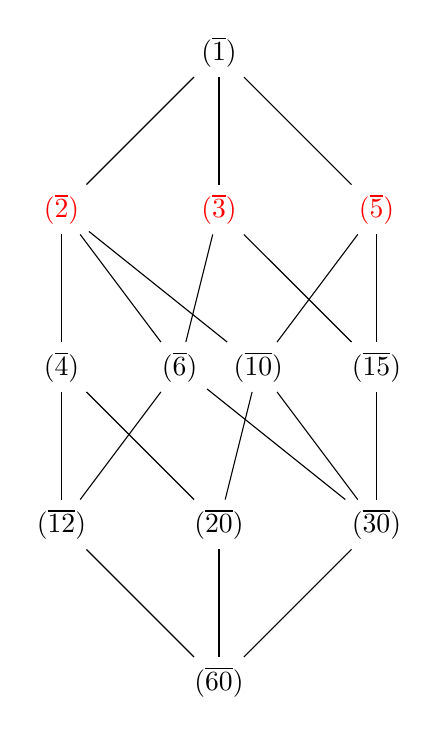
\begin{tikzpicture}
        % 设置节点
        \node (1) at (3,8) {$(\overline{1})$};
        \node (2) at (1,6) {$\color{red}(\overline{2})$};
        \node (3) at (3,6) {$\color{red}(\overline{3})$};
        \node (5) at (5,6) {$\color{red}(\overline{5})$};
        \node (4) at (1,4) {$(\overline{4})$};
        \node (6) at (2.5,4) {$(\overline{6})$};
        \node (10) at (3.5,4) {$(\overline{10})$};
        \node (15) at (5,4) {$(\overline{15})$};
        \node (12) at (1,2) {${(\overline{12})}$};
        \node (20) at (3,2) {${(\overline{20})}$};
        \node (30) at (5,2) {${(\overline{30})}$};
        \node (60) at (3,0) {$(\overline{60})$};

        % 画包含关系的边
        \draw[-] (1) -- (2);
        \draw[-] (1) -- (3);
        \draw[-] (1) -- (5);
        \draw[-] (2) -- (4);
        \draw[-] (2) -- (6);
        \draw[-] (2) -- (10);
        \draw[-] (3) -- (6);
        \draw[-] (3) -- (15);
        \draw[-] (4) -- (12);
        \draw[-] (4) -- (20);
        \draw[-] (6) -- (12);
        \draw[-] (6) -- (30);
        \draw[-] (5) -- (10);
        \draw[-] (5) -- (15);
        \draw[-] (10) -- (20);
        \draw[-] (10) -- (30);
        \draw[-] (15) -- (30);
        \draw[-] (12) -- (60);
        \draw[-] (30) -- (60);
        \draw[-] (20) -- (60);
    \end{tikzpicture}
    \caption{Ideals of $\mathbb{Z}/60\mathbb{Z}$ }
    \label{figure: Z/(60)}
\end{figure}

\end{solution}

\setcounter{pb}{20} 
\begin{problem}
    Let $ G $ be an abelian group with a finite set of generators which is periodic in the sense that all of its elements have finite order. Show that $ G $ is finite.
\end{problem}

\begin{solution}
    Let $\{g_{1},\dots,g_{m}\}$ be a  periodic set of generators. Then it suffices to show that
        \[
            g_{1}^{k_{1}}g_{2}^{k_{2}}\cdots g_{m}^{k_{m}},\quad k_{i}\in\mathbb{Z}
        \]
    have only finitely many results, since $G$ is Abelian. By periodicity, we can restrict $|k_{i}|\leq k$ for some $k\in\mathbb{Z}$ and then 
    we have $|G|\leq k^{m}$.
\end{solution}

\setcounter{pb}{24}
\begin{problem}
    Verify that for $ a, b \in \mathbb{R} $, the mapping  
    \[
    a + b \sqrt{-1} \mapsto 
    \begin{pmatrix}
        a & b \\
        -b & a
    \end{pmatrix}
    \]
    is an isomorphism of $\mathbb{C}$ with a subring of $ M_2(\mathbb{R}) $.
\end{problem}

\begin{solution}
    Denote the mapping by $\varphi$, then it is additive. For multiplication, 
        \[
            \begin{split}
                \varphi((a+b\sqrt{-1})(c+d\sqrt{-1}))
                &=\varphi(a c-b d+(a d+b c)\sqrt{-1})\\
                &=
                \begin{pmatrix}
                    a c-b d& a d+b c\\
                    a d+b c& a c-b d
                \end{pmatrix}
                =
                \begin{pmatrix}
                    a & b \\
                    -b & a
                \end{pmatrix}
                \begin{pmatrix}
                    c & d \\
                    -d & c            
                \end{pmatrix}\\
                &=\varphi(a+b\sqrt{-1})\varphi(c+d\sqrt{-1}).
            \end{split}
        \]
    Thus, $\varphi\colon \mathbb{C}\to\varphi(\mathbb{C})$ is an isomorphism, where $\varphi(\mathbb{C})=\Bigg\{
    \begin{bmatrix}
        a&b\\-b&a
    \end{bmatrix}:a,b\in\mathbb{R}\Bigg\}$ is a subring of $M_{2}(\mathbb{R})$. 
\end{solution}

% \setcounter{pb}{27}
% \begin{problem}
%     For a commutative ring with unit, show that the intersection of prime ideals is the set of nilpotent elements.
% \end{problem}